%%%%%%%%%%%%%%%%%%%%%%%%%%%%%%%%%%%%%%%%%
% Jacobs Landscape Poster
% LaTeX Template
% Version 1.1 (14/06/14)
%
% Created by:
% Computational Physics and Biophysics Group, Jacobs University
% https://teamwork.jacobs-university.de:8443/confluence/display/CoPandBiG/LaTeX+Poster
% 
% Further modified by:
% Nathaniel Johnston (nathaniel@njohnston.ca)
%
% This template has been downloaded from:
% http://www.LaTeXTemplates.com
%
% License:
% CC BY-NC-SA 3.0 (http://creativecommons.org/licenses/by-nc-sa/3.0/)
%
%%%%%%%%%%%%%%%%%%%%%%%%%%%%%%%%%%%%%%%%%

%----------------------------------------------------------------------------------------
%	PACKAGES AND OTHER DOCUMENT CONFIGURATIONS
%----------------------------------------------------------------------------------------

\documentclass[final]{beamer}

\usepackage[scale=1.24]{beamerposter} % Use the beamerposter package for laying out the poster

\usepackage[utf8]{inputenc}
\usepackage[english]{babel}

\usepackage{wrapfig}

\usetheme{confposter} % Use the confposter theme supplied with this template

\setbeamercolor{block title}{fg=ngreen,bg=white} % Colors of the block titles
\setbeamercolor{block body}{fg=black,bg=white} % Colors of the body of blocks
\setbeamercolor{block alerted title}{fg=white,bg=dblue!70} % Colors of the highlighted block titles
\setbeamercolor{block alerted body}{fg=black,bg=dblue!10} % Colors of the body of highlighted blocks
% Many more colors are available for use in beamerthemeconfposter.sty

%-----------------------------------------------------------
% Define the column widths and overall poster size
% To set effective sepwid, onecolwid and twocolwid values, first choose how many columns you want and how much separation you want between columns
% In this template, the separation width chosen is 0.024 of the paper width and a 4-column layout
% onecolwid should therefore be (1-(# of columns+1)*sepwid)/# of columns e.g. (1-(4+1)*0.024)/4 = 0.22
% Set twocolwid to be (2*onecolwid)+sepwid = 0.464
% Set threecolwid to be (3*onecolwid)+2*sepwid = 0.708

\newlength{\sepwid}
\newlength{\onecolwid}
\newlength{\twocolwid}
\newlength{\threecolwid}
\setlength{\paperwidth}{48in} % A0 width: 46.8in
\setlength{\paperheight}{36in} % A0 height: 33.1in
\setlength{\sepwid}{0.024\paperwidth} % Separation width (white space) between columns
\setlength{\onecolwid}{0.22\paperwidth} % Width of one column
\setlength{\twocolwid}{0.464\paperwidth} % Width of two columns
\setlength{\threecolwid}{0.708\paperwidth} % Width of three columns
\setlength{\topmargin}{-0.5in} % Reduce the top margin size
%-----------------------------------------------------------

\usepackage{graphicx}  % Required for including images

\usepackage{booktabs} % Top and bottom rules for tables

%----------------------------------------------------------------------------------------
%	TITLE SECTION 
%----------------------------------------------------------------------------------------

\title{Predicting I/O performance in HPC using Artificial Neural Networks} % Poster title

\author{Jan Fabian Schmid and Julian Kunkel} % Author(s)

\institute{Universität Hamburg} % Institution(s)

%----------------------------------------------------------------------------------------

\begin{document}

\addtobeamertemplate{block end}{}{\vspace*{2ex}} % White space under blocks
\addtobeamertemplate{block alerted end}{}{\vspace*{2ex}} % White space under highlighted (alert) blocks

\setlength{\belowcaptionskip}{2ex} % White space under figures
\setlength\belowdisplayshortskip{2ex} % White space under equations

\begin{frame}[t] % The whole poster is enclosed in one beamer frame

\begin{columns}[t] % The whole poster consists of three major columns, the second of which is split into two columns twice - the [t] option aligns each column's content to the top

\begin{column}{\sepwid}\end{column} % Empty spacer column

\begin{column}{\onecolwid} % The first column

%----------------------------------------------------------------------------------------
%	GOALS
%----------------------------------------------------------------------------------------

\begin{alertblock}{Goals}

%The goals of this work were:

\begin{itemize}
\item Gain knowledge about the storage system of a super computer for the development of computational models in the future
\item Find an artificial neural network that is reliable in predicting performance of HPC-IO with sufficient quality
\item Extract information about the I/O-paths for file access used by the storage system
\end{itemize}

\end{alertblock}

%----------------------------------------------------------------------------------------
%	INTRODUCTION
%----------------------------------------------------------------------------------------

\begin{block}{Introduction}
	
There is a need for tools that help users to implement efficient input/output (I/O) in their software, because this is a complex and time-consuming task. Finding the best access parameters and patterns is difficult, mainly because of the use of complex parallel storage systems in HPC.
%Currently users have to optimize their programs at great expense to each system individually without much assistance.
For the development of tools to support the implementation of efficient I/O the availability of a computational model of the storage system is key.\medskip

We analysed the storage system of a super computer and tried to find a good predictor for its I/O-performance using artificial neural networks (ANNs).
A hypothesis was then made: \textbf{The I/O-path determines the performance of a file access.}
The I/O-performance of a file access is more dependent on the processing in the storage system than on the access size for example.\medskip

To test our hypothesis we used ANNs with different input information for the prediction of access times.
For the use of I/O-paths as input information for the ANNs we developed a method to compute an approximation of the different I/O-paths used in an benchmark-test.
%This statement requires citation \cite{Smith:2012qr}.

\end{block}

%------------------------------------------------

%\begin{figure}
%\includegraphics[width=0.8\linewidth]{placeholder.jpg}
%\caption{Figure caption}
%\end{figure}

%----------------------------------------------------------------------------------------

\end{column} % End of the first column

\begin{column}{\sepwid}\end{column} % Empty spacer column

\begin{column}{\onecolwid} % The sec column
	
\begin{block}{Artificial Neural Networks}
	
	ANNs are bio-inspired function approximators.
	
	%\begin{wrapfigure}{r}{0.6\textwidth}
	%	\begin{center}
	%		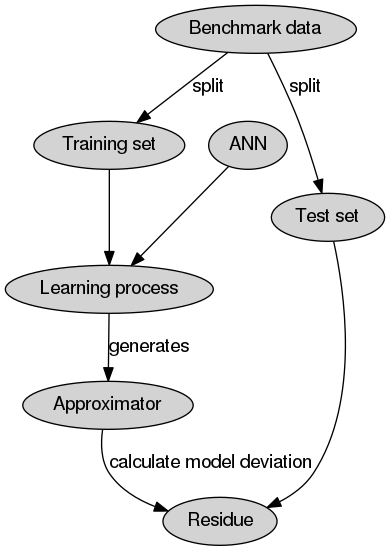
\includegraphics[height=1\textwidth]{src/tupel1.png}
	%	\end{center}
	%	\caption{G}
	%	\label{fig:evo}
	%\end{wrapfigure}
	
	An ANN is able to approximate a function that maps given input vectors on their associated output vectors.
	This is done by adapting the connection weights in the network using gradient decent during a supervised learning process (backpropagation).
	With appropriate topology ANNs are able to approximate any continuous functions on compact subsets of $\mathbb{R}^n$ \cite{cybenko:mcss}.
	
	%\begin{figure}
	%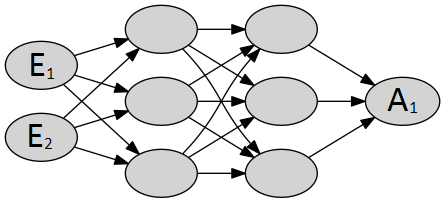
\includegraphics[height=0.3\linewidth]{src/netz.png}
	%\caption{small feedforward-network}
	%\end{figure}
	
\end{block}

\begin{block}{Model of the I/O-path}
	
	The processing of a file access in the storage system can be viewed using the I/O-path.
	That is the path from the invoking processor to the storage medium that contains the necessary data.
	The resulting access time of the process is then dependent on the depth of the path, because the further the path goes into the storage system, the the slower the storage media get.
	While the first storage levels (Caches) are very quick to respond, the main memory is already magnitudes slower, the same applies for the step into the parallel storage system that is connected via network to the computer nodes.\medskip
	
	As can be seen in figure \ref{read_rnd} the access times increase with access sizes.
	However a phenomenon that can be explained with the I/O-path model can be seen as well; access times of measurements with same parameter values are split into several groups of durations. Different I/O-paths were used for file accesses in these groups, which led to a step in the magnitude of the access time. 
	
	\begin{figure}
		\label{read_rnd}
		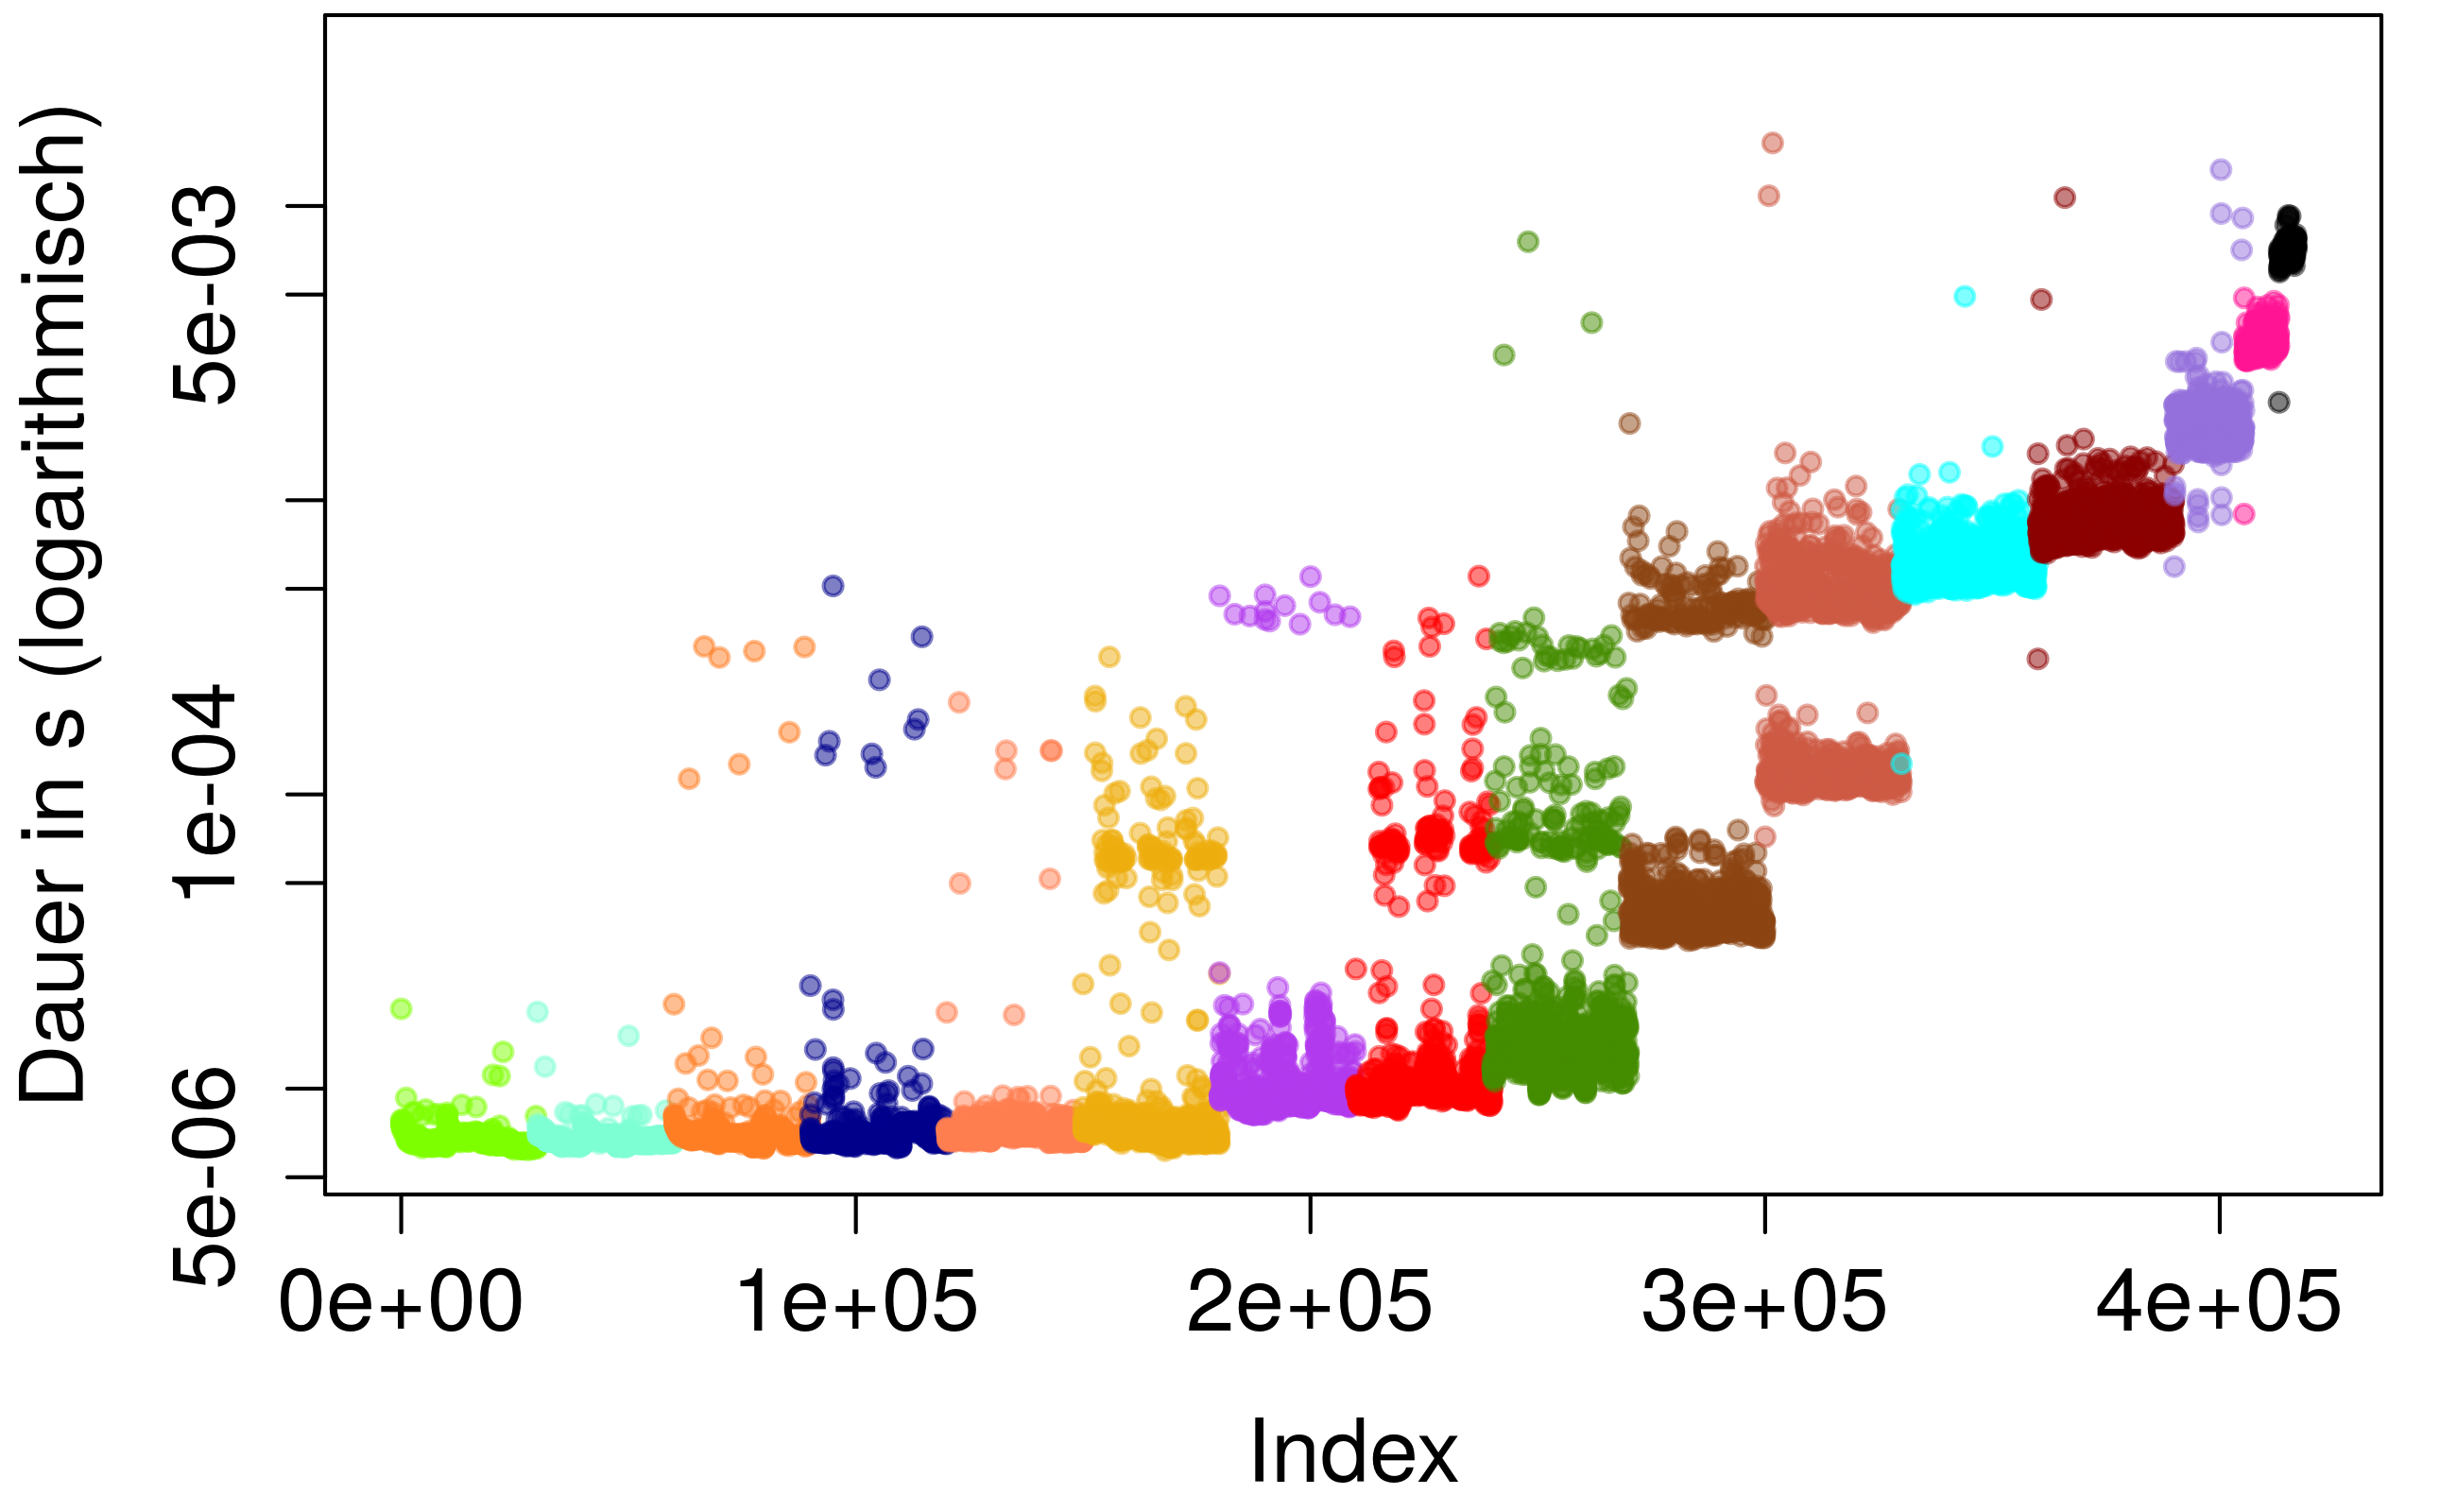
\includegraphics[width=0.8\linewidth]{src/plot_SizeSorted_log_read_seq.png}
		\caption{Access times of measurements with increasing access sizes. The sizes increase from left to right, all measurements with the same size have the same color.}
	\end{figure}
	
	%\begin{figure}
	%	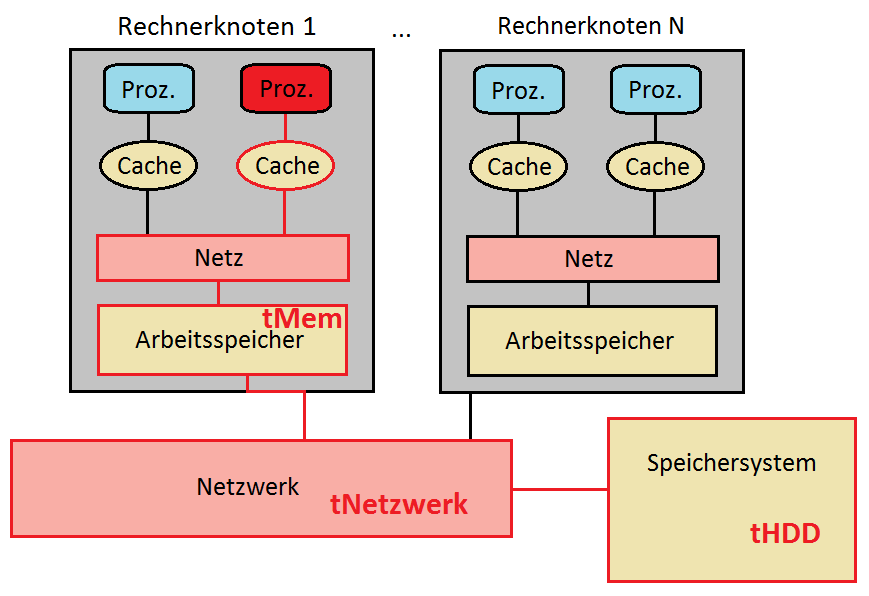
\includegraphics[width=1\linewidth]{src/rechnerknoten_ea_pfad.png}
	%	\caption{Sketch of the storage system in a super computer}
	%\end{figure}
	
\end{block}
	
\end{column} % End of the sec column

\begin{column}{\sepwid}\end{column} % Empty spacer column

\begin{column}{\onecolwid} % The 3 column
	
\begin{block}{Benchmark-Tests}
	
	The measurements were done on the super computer Mistral of the DKRZ (Deutsches Klimarechenzentrum).
	%Mistral operates with the parallel distributed file system Lustre and consist of over 1500 computing nodes and 30 petabyte storage.
	Two different use cases were tested: Sequential and random file access.
	Access sizes varied from 1\,B to 16\,MiB.
	
\end{block}

\begin{block}{Models}
	
	As baseline model linear regression was used for a simple mapping of access size to access time of measurements.
	Three models with different input information utilizing ANNs were then used to predict the access times.
	Every ANN-model received access size, file offset and access type as input.
	Additionally one model receives information about the past data throughputs of the system, this can be used to model time dependencies of the I/O-performance in the system (see figure \ref{time_dep}). Another model receives error classes as input.
	
		\begin{figure}
			\label{time_dep}
			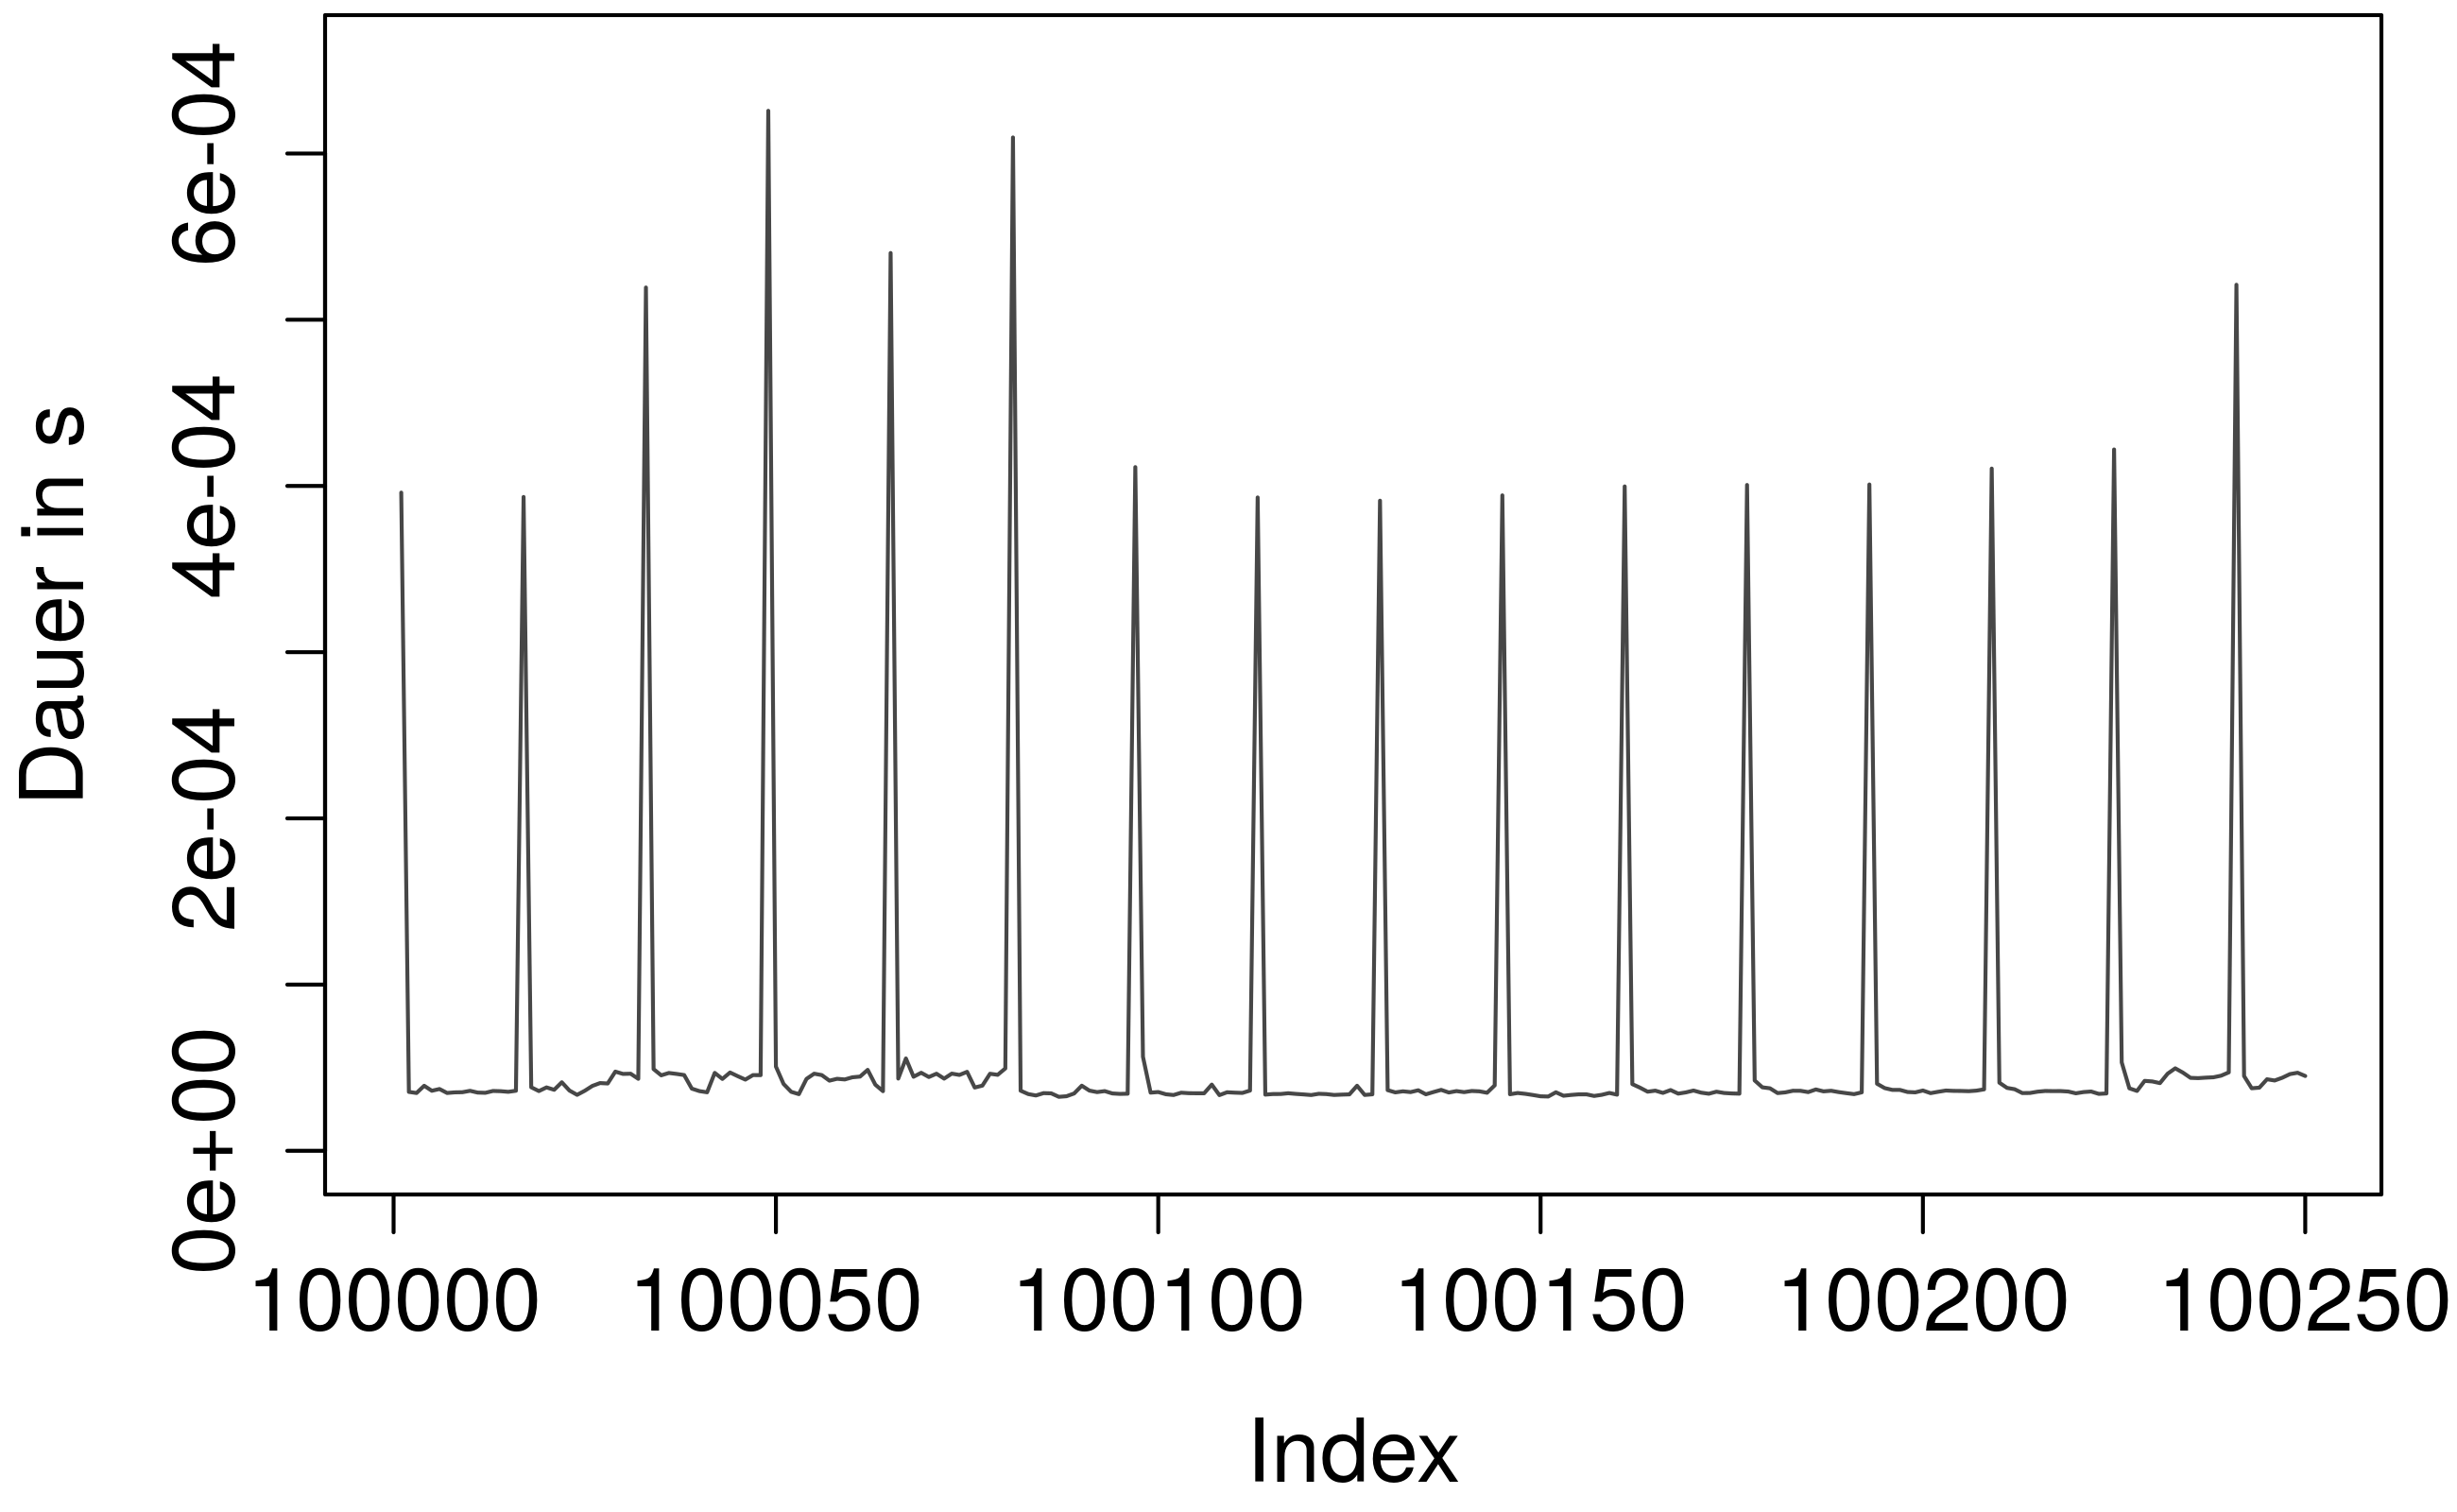
\includegraphics[width=0.8\linewidth]{src/plot_From100001to100250_read_seq.png}
			\caption{A small sequence of file accesses with same parameters. Peaks in the access times occure regularly.}
		\end{figure}
	
\end{block}

\begin{block}{Error Classes}
	

	
\end{block}

\end{column} % End of the 3 column

\begin{column}{\sepwid}\end{column} % Empty spacer column

\begin{column}{\onecolwid} % The 4 column

\begin{block}{Results}
	
	Nam quis odio enim, in molestie libero. Vivamus cursus mi at nulla elementum sollicitudin. Nam quis odio enim, in molestie libero. Vivamus cursus mi at nulla elementum sollicitudin.
	Nam quis odio enim, in molestie libero. Vivamus cursus mi at nulla elementum sollicitudin. Nam quis odio enim, in molestie libero. Vivamus cursus mi at nulla elementum sollicitudin.
	
	
\end{block}

%----------------------------------------------------------------------------------------
%	CONCLUSION
%----------------------------------------------------------------------------------------

\begin{block}{Conclusion}

Nunc tempus venenatis facilisis. \textbf{Curabitur suscipit} consequat eros non porttitor. Sed a massa dolor, id ornare enim. Fusce quis massa dictum tortor \textbf{tincidunt mattis}. Donec quam est, lobortis quis pretium at, laoreet scelerisque lacus. Nam quis odio enim, in molestie libero. Vivamus cursus mi at \textit{nulla elementum sollicitudin}.

\end{block}


%----------------------------------------------------------------------------------------
%	REFERENCES
%----------------------------------------------------------------------------------------

\begin{block}{References}

\nocite{*} % Insert publications even if they are not cited in the poster
\small{\bibliographystyle{unsrt}
\bibliography{sample}\vspace{0.75in}}

\end{block}

%----------------------------------------------------------------------------------------
%	ACKNOWLEDGEMENTS
%----------------------------------------------------------------------------------------

%\setbeamercolor{block title}{fg=red,bg=white} % Change the block title color
%
%\begin{block}{Acknowledgements}
%
%\small{\rmfamily{Nam mollis tristique neque eu luctus. Suspendisse rutrum congue nisi sed convallis. Aenean id neque dolor. Pellentesque habitant morbi tristique senectus et netus et malesuada fames ac turpis egestas.}} \\
%
%\end{block}

%----------------------------------------------------------------------------------------
%	CONTACT INFORMATION
%----------------------------------------------------------------------------------------

\setbeamercolor{block alerted title}{fg=black,bg=norange} % Change the alert block title colors
\setbeamercolor{block alerted body}{fg=black,bg=white} % Change the alert block body colors

\begin{alertblock}{Contact Information}

\begin{itemize}
\item Web: \href{http://wr.informatik.uni-hamburg.de}{http://wr.informatik.uni-hamburg.de}
\item Email: \href{mailto:2schmid@informatik.uni-hamburg.de}{2schmid@informatik.uni-hamburg.de}
\end{itemize}

\end{alertblock}

\begin{flushright}
\begin{tabular}{r}

\includegraphics[width=0.2\linewidth]{src/2000px-Unihamburg-logo.png} % & \hfill & \includegraphics[width=0.4\linewidth]{logo.png}
\end{tabular}
\end{flushright}

%----------------------------------------------------------------------------------------

\end{column} % End of the 4 column

\end{columns} % End of all the columns in the poster

\end{frame} % End of the enclosing frame

\end{document}
